%% abtex2-modelo-projeto-pesquisa.tex, v-1.9.6 laurocesar
%% Copyright 2012-2016 by abnTeX2 group at http://www.abntex.net.br/ 
%%
%% This work may be distributed and/or modified under the
%% conditions of the LaTeX Project Public License, either version 1.3
%% of this license or (at your option) any later version.
%% The latest version of this license is in
%%   http://www.latex-project.org/lppl.txt
%% and version 1.3 or later is part of all distributions of LaTeX
%% version 2005/12/01 or later.
%%
%% This work has the LPPL maintenance status `maintained'.
%% 
%% The Current Maintainer of this work is the abnTeX2 team, led
%% by Lauro César Araujo. Further information are available on 
%% http://www.abntex.net.br/
%%
%% This work consists of the files abntex2-modelo-projeto-pesquisa.tex
%% and abntex2-modelo-references.bib
%%

% ------------------------------------------------------------------------
% ------------------------------------------------------------------------
% abnTeX2: Modelo de Projeto de pesquisa em conformidade com 
% ABNT NBR 15287:2011 Informação e documentação - Projeto de pesquisa -
% Apresentação 
% ------------------------------------------------------------------------ 
% ------------------------------------------------------------------------

\documentclass[
% -- opções da classe memoir --
article,			% indica que é um artigo acadêmico
12pt,				% tamanho da fonte
openright,			% capítulos começam em pág ímpar (insere página vazia caso preciso)
oneside,			% para impressão em recto. Oposto a twoside
%twoside,			% para impressão em recto e verso. Oposto a oneside
a4paper,			% tamanho do papel. 
% -- opções da classe abntex2 --
chapter=TITLE,		% títulos de capítulos convertidos em letras maiúsculas
section=TITLE,		% títulos de seções convertidos em letras maiúsculas
subsection=TITLE,	% títulos de subseções convertidos em letras maiúsculas
subsubsection=TITLE,% títulos de subsubseções convertidos em letras maiúsculas
subsubsubsection=TITLE, % títulos de subsubsubseções em letras maiúsculas
% -- opções do pacote babel --
english,			% idioma adicional para hifenização
%french,			% idioma adicional para hifenização
%spanish,			% idioma adicional para hifenização
brazil,				% o último idioma é o principal do documento
]{abntex2}

% ---
% PACOTES
% ---

% ---
% Pacotes fundamentais 
% ---
\usepackage{lmodern}			% Usa a fonte Latin Modern
\usepackage[T1]{fontenc}		% Selecao de codigos de fonte.
\usepackage[utf8]{inputenc}		% Codificacao do documento (conversão automática dos acentos)
\usepackage{indentfirst}		% Indenta o primeiro parágrafo de cada seção.
\usepackage{color}				% Controle das cores
\usepackage{graphicx}			% Inclusão de gráficos
\usepackage{microtype} 			% para melhorias de justificação
%\usepackage[none]{hyphenat} 			% Desativa ifenização
% ---

% ---
% Pacotes adicionais, usados apenas no âmbito do Modelo Canônico do abnteX2
% ---
\usepackage{lipsum}				% para geração de dummy text
% ---

% ---
% Pacotes de citações
% ---
\usepackage[brazilian,hyperpageref]{backref}	 % Paginas com as citações na bibl
\usepackage[alf]{abntex2cite}	% Citações padrão ABNT

% --- 
% CONFIGURAÇÕES DE PACOTES
% --- 

% ---
% Configurações do pacote backref
% Usado sem a opção hyperpageref de backref
\renewcommand{\backrefpagesname}{Citado na(s) página(s):~}
% Texto padrão antes do número das páginas
\renewcommand{\backref}{}
% Define os textos da citação
\renewcommand*{\backrefalt}[4]{%
    \ifcase #1 %
        Nenhuma citação no texto.%
        \or
        Citado na página #2.%
    \else
        Citado #1 vezes nas páginas #2.%
\fi}%
% ---

% ---
% Configurações do modelo IFPR
\usepackage{abntex2ifpr}

% ---
% Informações de dados para CAPA, FOLHA DE ROSTO e FOLHA DE APROVAÇÃO
% ---
\titulo{Modelo para trabalhos acadêmicos no IFPR com \abnTeX}
\autor{Mateus Mercer e Equipe \abnTeX}
\local{Londrina}
\data{2018}
\orientador{INSIRA O ORIENTADOR}
%\coorientador{INSIRA O COORIENTADOR}
\convidadoum{INSIRA O CONVIDADO 1}
\convidadodois{INSIRA O CONVIDADO 2}
\curso{Curso Superior de Tecnologia em Análise e Desenvolvimento de Sistemas}
% O preambulo deve conter o tipo do trabalho, o objetivo, 
% o nome da instituição e a área de concentração 
\preambulo{Trabalho de Conclusão de Curso apresentado ao \imprimircurso do Instituto 
    Federal do Paraná \@\textendash\@ Campus Londrina, como 
requisito parcial de avaliação.}
% ---

% ---
% Configurações de aparência do PDF final

% alterando o aspecto da cor azul
\definecolor{blue}{RGB}{41,5,195}

% informações do PDF
\makeatletter
\hypersetup{%
    %pagebackref=true,
    pdftitle={\@title}, 
    pdfauthor={\@author},
    pdfsubject={\imprimirpreambulo},
    pdfcreator={LaTeX with abnTeX2},
    pdfkeywords={abnt}{latex}{abntex}{abntex2}{projeto de pesquisa}, 
    colorlinks=false,       		% false: boxed links; true: colored links
    linkcolor=blue,          	% color of internal links
    citecolor=blue,        		% color of links to bibliography
    filecolor=magenta,      		% color of file links
    urlcolor=blue,
    bookmarksdepth=4
}
\makeatother
% --- 

% --- 
% Espaçamentos entre linhas e parágrafos 
% --- 

% O tamanho do parágrafo é dado por:
\setlength{\parindent}{1.3cm}

% Controle do espaçamento entre um parágrafo e outro:
\setlength{\parskip}{0.2cm}  % tente também \onelineskip

% ---
% compila o indice
% ---
\makeindex
% ---

% ---
% Aonde as imagens estao
% ---
\graphicspath{{imagens/}}
% ---

% ----
% Início do documento
% ----
\begin{document}

% Seleciona o idioma do documento (conforme pacotes do babel)
%\selectlanguage{english}
\selectlanguage{brazil}

% Retira espaço extra obsoleto entre as frases.
\frenchspacing 

% ----------------------------------------------------------
% ELEMENTOS PRÉ-TEXTUAIS
% ----------------------------------------------------------
% \pretextual

% ---
% Capa
% ---
\imprimircapa
% ---

% ---
% Folha de rosto
% ---
\imprimirfolhaderosto
% ---

% ---
% Inserir folha de aprovação
% ---

% Isto é um exemplo de Folha de aprovação, elemento obrigatório da NBR
% 14724/2011 (seção 4.2.1.3). Você pode utilizar este modelo até a aprovação
% do trabalho. Após isso, substitua todo o conteúdo deste arquivo por uma
% imagem da página assinada pela banca com o comando abaixo:
%
% \begin{folhadeaprovacao}
% \includepdf{folhadeaprovacao_final.pdf}
% \end{folhadeaprovacao}
%
\begin{folhadeaprovacao}
    \begin{center}
        \begin{center}
            \ABNTEXchapterfont\bfseries FOLHA DE APROVAÇÃO
            \par
            \vspace*{1.5cm}
            {\normalfont\ABNTEXchapterfontsize\MakeUppercase\imprimirautor}
            \vspace*{1.5cm}
            \par
            {\normalfont\ABNTEXchapterfontsize\MakeUppercase\imprimirtitulo}
        \end{center}
        \vspace*{\fill}

        \hspace{.45\textwidth}
        \begin{minipage}{.5\textwidth}
            \imprimirpreambulo
        \end{minipage}%
        \vspace*{\fill}
    \end{center}

    \assinatura{\textbf{\imprimirorientador} \\ Orientador} 
    \assinatura{\textbf{\imprimirconvidadoum} \\ Convidado 1}
    \assinatura{\textbf{\imprimirconvidadodois} \\ Convidado 2}
    %\assinatura{\textbf{Professor} \\ Convidado 3}
    %\assinatura{\textbf{Professor} \\ Convidado 4}

    \vspace{3cm}
    \begin{center}
        \imprimirlocal, 22 de Janeiro de 1999.
    \end{center}

    \pagebreak
\end{folhadeaprovacao}
% ---

% ---
% NOTA DA ABNT NBR 15287:2011, p. 4:
%  ``Se exigido pela entidade, apresentar os dados curriculares do autor em
%     folha ou página distinta após a folha de rosto.''
% ---

% ---
% inserir lista de ilustrações
% ---
\pdfbookmark[0]{\listfigurename}{lof}
\listoffigures*
\cleardoublepage
% ---

% ---
% inserir lista de tabelas
% ---
\pdfbookmark[0]{\listtablename}{lot}
\listoftables*
\cleardoublepage
% ---

% ---
% inserir lista de abreviaturas e siglas
% ---
\begin{siglas}
\item[ABNT] Associação Brasileira de Normas Técnicas
\item[abnTeX] ABsurdas Normas para TeX
\end{siglas}
% ---

% ---
% inserir lista de símbolos
% ---
\begin{simbolos}
\item[$ \Gamma $] Letra grega Gama
\item[$ \Lambda $] Lambda
\item[$ \zeta $] Letra grega minúscula zeta
\item[$ \in $] Pertence
\end{simbolos}
% ---

% ---
% inserir o sumario
% ---
\pdfbookmark[0]{\contentsname}{toc}
\tableofcontents*
\cleardoublepage
% ---


% ----------------------------------------------------------
% ELEMENTOS TEXTUAIS
% ----------------------------------------------------------
\textual

% Introdução
\section{Introdução}

\subsection{Contexto}

Há indícios que as Criptomoedas surgiram com o enfraquecimento do
dólar como padrão monetário internacional \cite{FAE2014}, diversas
tecnologias surgiram ao longo do tempo, que revolucionaram como as
instituições monetárias, sejam elas governamentais ou não, interagem
com essas moedas sem lastros \cite{Said2017}. 
% TODO: Trocara referência para gazeta do povo

Softwares e Hardwares foram criados para gerenciar essas novas
tecnologias, a mais famosa é o Bitcoin. O principal objetivo do
Bitcoin é transferir tokens de valor monetário evitando a dependência
entre uma instituição intermediaria para validar as transações
\cite{Nakamoto2008}. Essa validação é feita pelo Blockchain, onde
existe uma lista de transações que necessitam ser, de maneira
criptografada, validadas \cite{Economist2015}.

Quando um bloco de transações é validado, quem validou recebe uma
quantia determinada de Bitcoin, minerar essa Criptomoeda nada mais é
que continuar as transações, incentivando novos mineradores. Em 2015,
foi estimado que mais de cem mil nodes (computadores na rede) estavam
minerando bitcoin \cite{Coin2015}. O Bitcoin muitas vezes não é uma
moeda viável para ser minerada em uma CPU de um computador doméstico
\cite{Bitcoins2018}.

Logo, existem outras alternativas de Criptomoedas que podem ser
mineradas em uma GPU ou CPU\@. Essa detecção atualmente não é feita
automaticamente por uma distribuição Linux. 

\subsection{Problema}

% TODO: Dificuldade de instalar o algoritmo correto par N moeda.
% Dificuldade para fazer o reconhecimento de placas gráficas.
% Falta de uma distribuição específica para isso. Suporte para a
% distribuição.
% TODO: Citação do distrorank
Fazer a configuração para uma distribuição Linux é um trabalho
repetitivo e que demanda tempo. Atualmente, as distribuições mais
populares automatizam o processo de instalação, configuração e
atualização. Porém, esta configuração é feita para um objetivo de uso
genérico, não para a mineração de Criptomoedas.

Para que um Node comece a minerar uma Criptomoeda, existe a
necessidade de configurar os seguintes componentes: (a) Os drivers de
vídeo; (b) O software para a mineração; (c) Configuração e inserção de
dados no software de mineração e (e) a criação ou configuração de uma
carteira. 

A distribuição Ethos é uma alternativa comercial para minerar
Criptomoedas, porém a configuração e instalação de drivers deve ser
feita manualmente \cite{EthOS2018}. A criação de uma distribuição
Linux genérica especifica para fazer esta detecção facilitaria muito o
trabalho de alguém que precisa configurar o software em um hardware de
alto desempenho.

% TODO: Referência bitcoin só ser lucrativo em grandes data centers
% TODO: Referência algoritmo Etash
Não é todo hardware que pode minerar uma Criptomoeda de maneira
lucrativa. O Bitcoin com o passar dos anos virou uma Criptomoeda que
só é possível ser minerada lucrativamente em grandes data centers com
hardwares específicos para o seu algoritmo. O Etash, utiliza um
algoritmo específico que somente permite a mineração lucrativa em
GPUs. Fazer esta detecção entre capacidade de hardware e Criptomoeda
não é um requisito que as distribuições atuais conseguem suprir.
% TODO: Referências???

\subsection{Objetivos}
% TODO: Remover seções geral e específico. Deixar somente parágrafos

\subsubsection{Geral}

Personalizar uma distribuição Linux capaz de automatizar a
configuração do hardware do equipamento para otimizar o tempo de
instalação do usuário.

\subsubsection{Específicos}

\begin{itemize} 

    \item Pesquisar drivers genéricos que funcionam em
        hardwares de alto desempenho;

    \item Personalizar uma distribuição Linux para a automatização da
        instalação dos drivers genéricos;

    \item Pesquisar diferentes Criptomoedas e suas vantagens e
        desvantagens em diferentes hardwares;

    \item Encontrar as melhores alternativas de softwares em termos de
        praticidade e tempo;

    \item Desenvolver a distribuição;

    \item Fazer um comparativo da velocidade de instalação entre a
distribuição e uma instalação manual.

\end{itemize}

\subsection{Método}

\subsection{Estrutura}

\section{Revisão de Literatura}

\subsection{Criptomoedas}

As Criptomoedas são um sistema descentralizado e independente de uma
instituição financeira. Sua facilidade de uso tornou as taxas de
transações cambiais menores, além de aumentar a velocidade com que
essas transações eram efetivadas. Isto chamou muito a atenção de
investidores, o que levou a uma difusão desta tecnologia na nossa
sociedade \cite{Nakamoto2008, Prado2017}.

\subsubsection{Definição}

Uma Criptomoeda é um sistema \emph{peer-to-peer} onde o controle da
moeda é feito por propriedades matemáticas e não por uma instituição
centralizada. Cada usuário é identificado por uma representação de sua
chave pública, também referenciada como endereço da carteira
\cite{Weber2012}. Para que um usuário faça uma transação, é necessário
que ele: (a) saiba o balanço de sua carteira, que é calculado por meio
do \emph{Blockchain}; (b) tenha o endereço da carteira de envio; e (c)
tenha a chave privada de sua carteira.

Em vez de existir um balanço em uma conta, existe uma lista de
transações feitas desde o início do sistema, chamada de
\emph{Blockchain} \cite{Weber2012}\label{def:blockchain}. O
\emph{Blockchain}, também referenciado como ``protocolo de
confiança'', usa a decentralização de uma instituição financeira como
uma medida de segurança. Cada transação deve ser validada
criptograficamente por vários nós de uma rede antes de entrar para o
\emph{Blockchain} \cite{LChicarino}. Diferente de um banco, que faz a
validação seguindo as sua próprias regras, sujeito a erros.

\subsubsection{Mineração}

Como dito anteriormente, na Seção~\ref{def:blockchain}, o
\emph{Blockchain} serve para validar uma transação. Somente existe uma
maneira de confirmar uma transação no \emph{Blockchain}: resolvendo um
``quebra cabeças'' criptográfico \cite{Weber2012}. Nessa resolução
criptográfica, um hash SHA-256 de um dado deve ser menor que um número
específico \cite{Dev2014}. Um hash, na linguagem comum, é um valor
único para um determinado dado.  Confirmar uma transação nada mais é
que descobrir este hash se utilizando da força bruta \cite{Arsov}.

A mineração serve para atualizar o \emph{Blockchain}, pelo qual nós
especiais, chamados de mineradores se encarregam em trabalhar de
maneira distribuída para fazer a validação de um conjunto de
transações, chamado de bloco. Toda vez que um cabeçalho válido é
gerado para o bloco, quem o valida recebe uma recompensa
\cite{LChicarino}. O incentivo na mineração é esta recompensa.

A recompensa também é definida como ``prova de trabalho''. Todos os
cabeçalhos de blocos novos são baseados no de blocos anteriores.
Portanto, para que o sistema seja atacado e corrompido, ou seja, para
que uma transação seja mudada manualmente, é necessário que o atacante
recalcule todos os blocos que foram gerados a partir do bloco que ele
quer modificar. Isto somente é possível se pelo menos $51\%$ do poder
computacional da rede inteira estiver nas mãos de quem a ataca
\cite{Nakamoto2008, Dev2014}.

A prova de trabalho também é um mecanismo de segurança. Diferentes
Criptomoedas utilizam diversos algoritmos para fazer as validações.
Logo, tornam-se necessários \emph{hardwares} específicos para que a
mineração seja feita. No Capítulo XXX apresentam-se os hardwares e
algoritmos mais comumente utilizados para este fim.
% TODO: Referência cruzada aqui

% TODO: Discutir sobre GPU ser melhor que CPU, etc.

\subsubsection{Rigs de Mineração}

Um rig de mineração é um sistema computacional que tem como
responsabilidade a mineração de uma Criptomoeda. Um computador com
hardwares gráficos de alto desempenho pode virar um rig de mineração
em tempo parcial. Também existe a possibilidade de várias placas
gráficas trabalharem em conjunto em um mesmo sistema. A
Figura~\ref{fig:rig_mineracao} é um exemplo de um rig de mineração com
múltiplas placas gráficas \cite{BitcoinWiki2015}.

\begin{figure}[!htbp]
    \caption{\label{fig:rig_mineracao}Um rig de mineração com 13 GPUs
    NVidia 1060}
    \begin{center}
        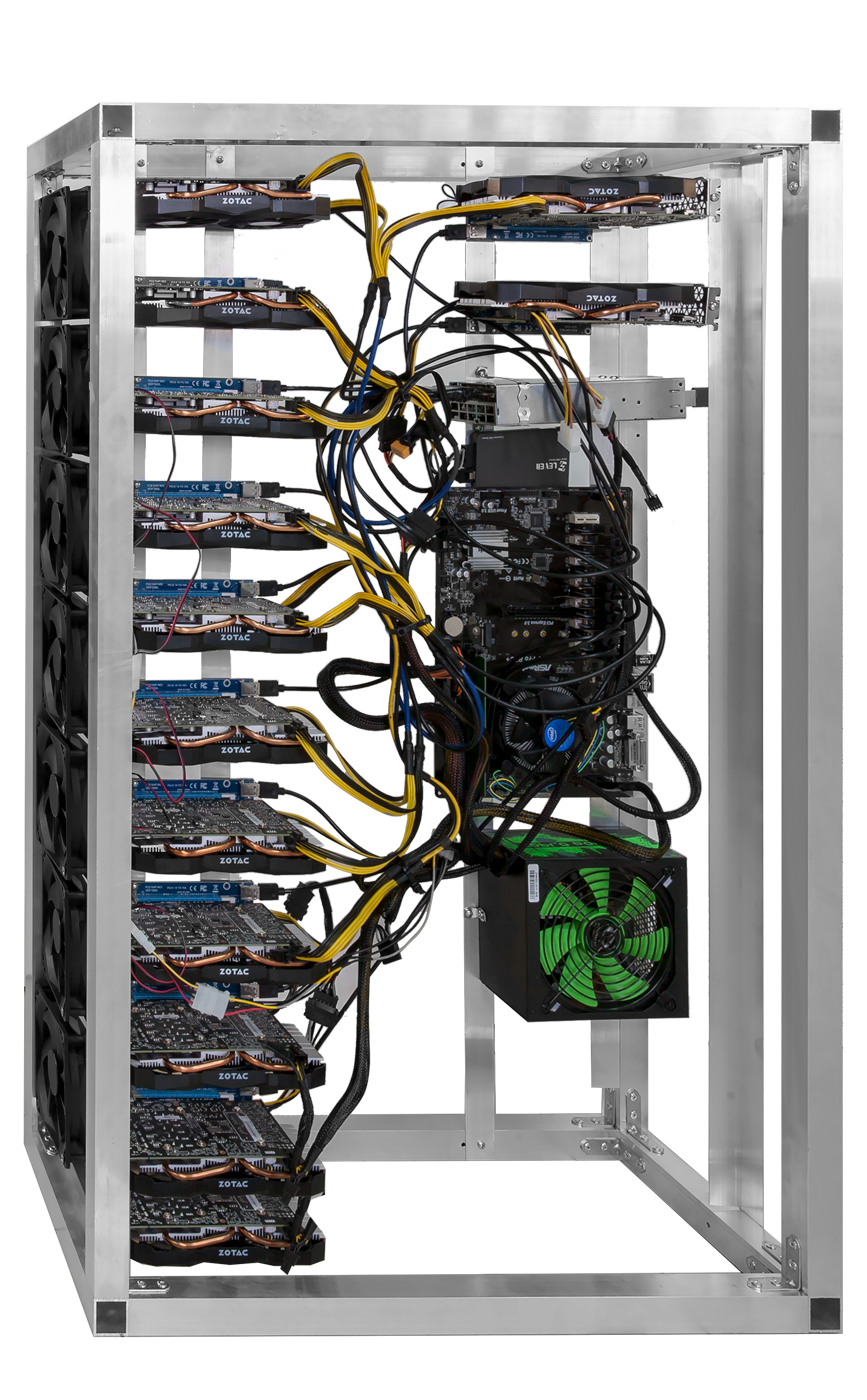
\includegraphics[width=.3\linewidth]{rig_mineracao.png}
    \end{center}
    \legend{Fonte: \url{https://mining.bg/13-gpu-mining-rig-nvidia-1060-3gb-8/}}
\end{figure}

\pagebreak

A medida utilizada para apresentar o desempenho de um rig de mineração
é ``hashes por segundo'', representado por $h/s$. \emph{Hardware} e
Criptomoeda são fatores que variam a quantidade de hashes por segundo.

\subsubsection{Litecoin}
% Descrever como o Litecoin surgiu e o que ele é
% Explicar como o litecoin tem um algoritmo de mineração que evita o
% uso por chips ASIC e FPGAs.
% TODO: Terminar esse parágrafo

Outras Criptomoedas, como o Litecoin e Etash, usam algoritmos que
dificultam a mineração por chips especializados, como ASICs e FPGAs.
Tornando a mineração somente lucrativa em CPUs ou GPUs
\cite{Weber2012}. Os Rigs de Mineração são valorizados dessa forma, já
que a mineração por GPU é muito mais lucrativa nessas Criptomoedas.

\subsubsection{Ethereum e Ethash}
% Descrever como o Ethereum surgiu e o que ele é
% Explicar como o Ethash também usa um algoritmo de mineração que
% evita o uso por chips ASIC e FPGAs.
% TODO: Terminar esse parágrafo

% ----------------------------------------------------------
% Referências bibliográficas (nome do arquivo de referencias, sem o
% ".bib"
% ----------------------------------------------------------
\pagebreak \bibliography{referencias}

\end{document}
